\subsection{Core ML and smartphone performance}

\begin{table}[t]
\caption{Runtime comparison for the mixed YOLO11n detector.}
\label{tab:runtime}
\centering
\begin{tabular}{lrrr}
\toprule
Runtime & Precision & ms/frame & FPS \\
\midrule
Mac PyTorch MPS & FP32 & 28.1 & 36 \\
Mac Core ML CPU & FP16 & 16.4 & 61 \\
Mac Core ML CPU+ANE & FP16 & 6.0 & 166 \\
iPhone CPU & FP16 & 11.7 & 86 \\
iPhone CPU+ANE & FP16 & 3.8 & 262 \\
\bottomrule
\end{tabular}
\end{table}

In the laptop evaluation, the FP16 Core ML export changes recall by at most
0.002 and counting MAE by 0.01 relative to FP32 PyTorch. The iPhone Neural
Engine runs the same package at a median 3.8 ms per frame
(Table~\ref{tab:runtime}). All 30 detections in the bundled samples match
between the Mac and the iPhone, with identical labels and a mean box IoU from
0.992 to 0.997 across the compute-unit settings. Compute units specify the
processors used for inference. Their outputs are not bit-identical: one
borderline fruit changes label between the CPU and Neural Engine settings.

\subsection{Effect of model size on accuracy and cost}
\label{sec:ladder}

\begin{table}[t]
\caption{The YOLO11 ladder trained under one protocol on Laboro. Counting MAE
is the best value over the confidence sweep, reported for all stages and for
fully ripe fruit alone, with the threshold that achieves it;
Table~\ref{tab:ladder-thresh} gives the same quantity at a fixed threshold.
Package size is
the FP16 Core ML artefact; load time is measured on the phone.}
\label{tab:ladder}
\centering
\begin{tabular}{lrrrrrr}
\toprule
Model & Params & GFLOPs & mAP & MAE & ripe MAE & MB \\
\midrule
YOLO11n & 2.58\,M & 6.3 & 0.706 & 0.963 & \textbf{0.590} & 5.4 \\
YOLO11s & 9.43\,M & 21.3 & 0.747 & 0.919 & 0.640 & 19.1 \\
YOLO11m & 20.03\,M & 67.7 & \textbf{0.782} & 0.882 & 0.627 & 40.3 \\
YOLO11l & 25.32\,M & 86.6 & 0.780 & \textbf{0.859} & 0.658 & 51.0 \\
YOLO11x & 56.88\,M & 194.4 & 0.774 & 0.874 & 0.602 & 114.1 \\
\bottomrule
\end{tabular}
\end{table}

\begin{figure}[t]
  \centering
  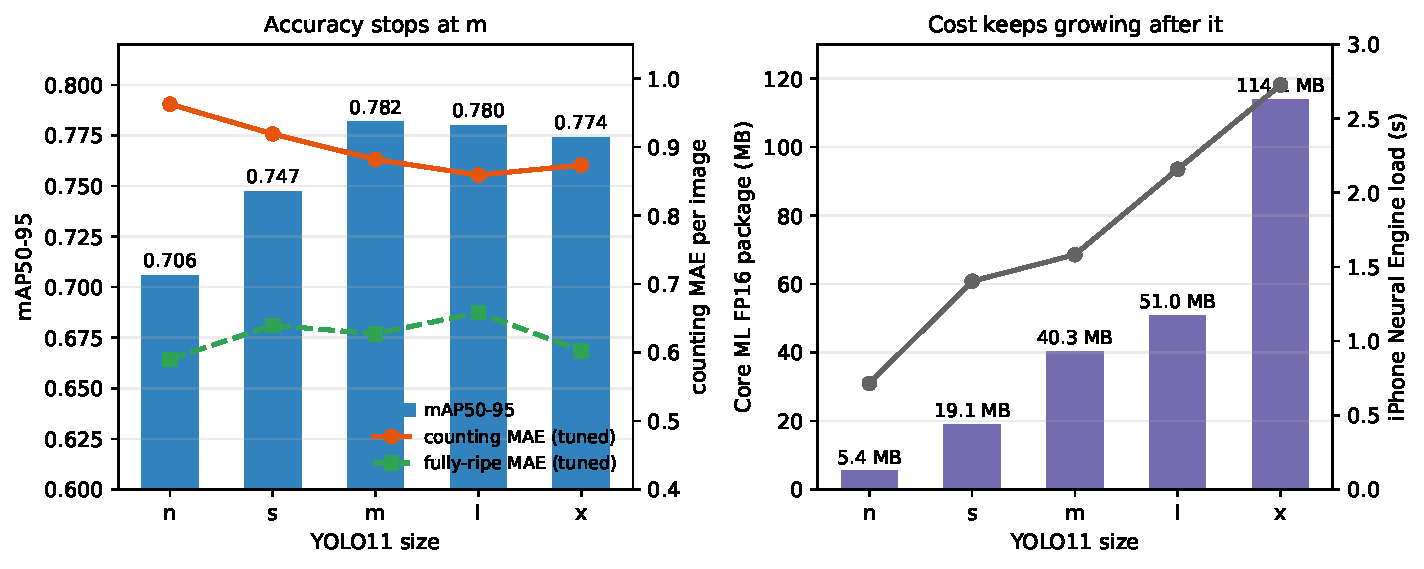
\includegraphics[width=\columnwidth]{size_accuracy.pdf}
  \caption{mAP50--95, tuned counting MAE, Core ML package size and model load
time across the five YOLO11 sizes.}
  \label{fig:size-accuracy}
\end{figure}

\begin{figure*}[t]
  \centering
  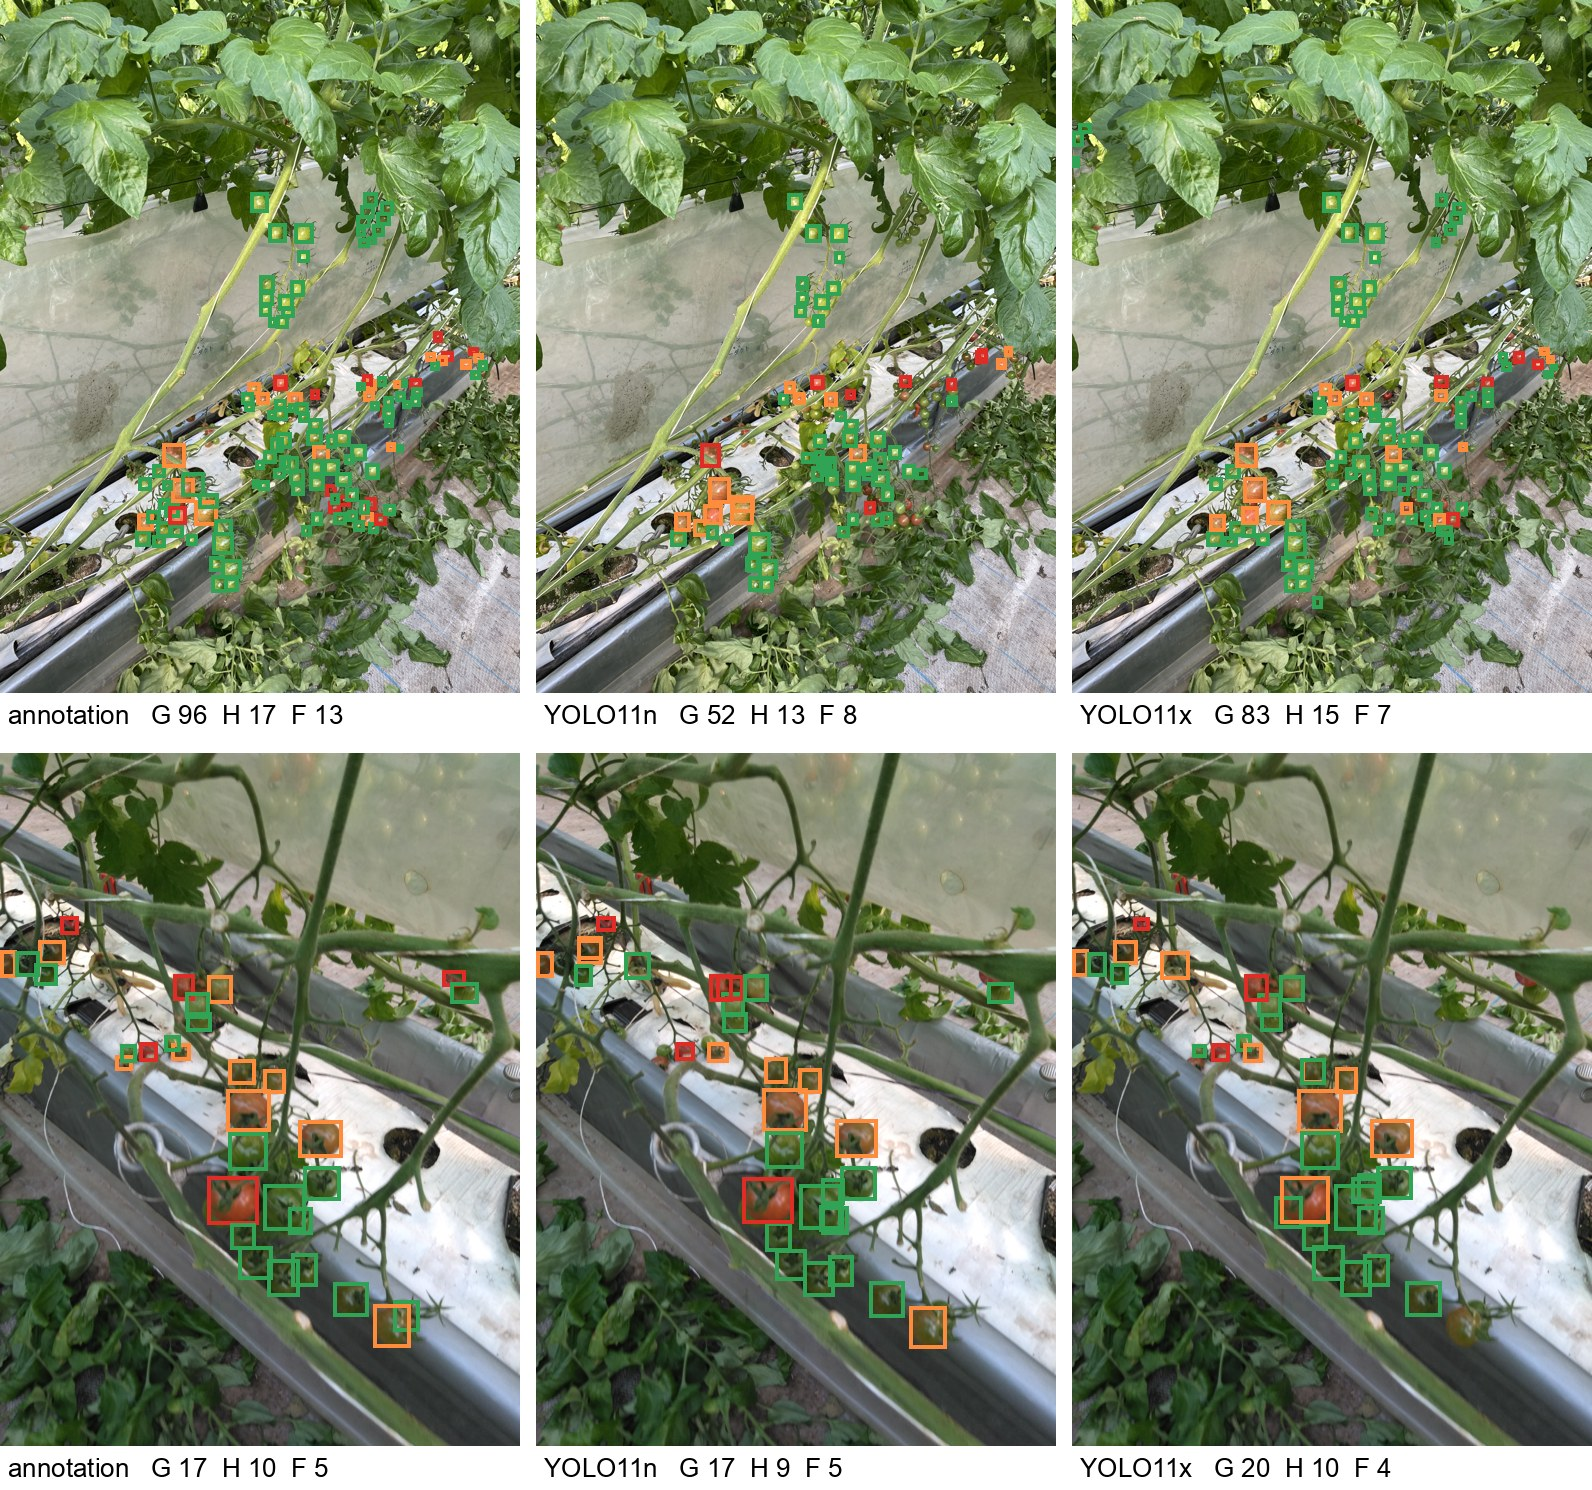
\includegraphics[width=0.92\textwidth]{detection_examples.jpg}
  \caption{Annotation (left), YOLO11n (centre) and YOLO11x (right) on the two
  Laboro validation frames with the most half-ripened fruit, at confidence
  0.25. Box colour is the maturity stage (green, orange for half-ripened, red
  for fully ripened); the counts of green (G), half-ripened (H) and fully
  ripened (F) fruit are printed under each panel. In the upper frame, which is
  dense with small fruit, YOLO11x finds far more of the green fruit than
  YOLO11n (83 against 52 of 96). In the lower frame both models count almost
  exactly, but YOLO11x labels the large red fruit in the centre half-ripened,
  while YOLO11n agrees with the annotation. The frames were selected
  automatically and are illustrations, not additional results.}
  \label{fig:detection-examples}
\end{figure*}

mAP50--95 rises from 0.706 for n to 0.747 for s and 0.782 for m. YOLO11l is
0.002 below m, and YOLO11x is 0.008 below m. Both differences are within the
variation that can be distinguished from a single seed
(Table~\ref{tab:ladder}). Tuned counting error continues to fall to 0.859 for l.
However, one seed does not support an ordering among m, l, and x.

Fully-ripe counting MAE does not decrease with model size. The best value on
the ladder is 0.590 for YOLO11n. Every larger model gives a value between 0.602
and 0.658. Higher overall detection accuracy therefore does not imply lower
fully-ripe counting error. A stage count depends first on detecting a fruit and
then on assigning its maturity stage. These results suggest that additional
capacity improved detection without improving the stage assignment.

From m to x, the Core ML package grows 2.8$\times$, Neural Engine latency grows
2.0$\times$, and model load time grows 1.7$\times$. The mAP does not increase
(Figure~\ref{fig:size-accuracy}).

\begin{table}[t]
\caption{Counting MAE at a fixed confidence of 0.25 and at the per-model best
threshold, both read from the same sweep over the same 161 validation images.
The best-threshold columns give the achieving confidence in brackets.}
\label{tab:ladder-thresh}
\centering
\begin{tabular}{lrlrl}
\toprule
 & \multicolumn{2}{c}{all stages} & \multicolumn{2}{c}{fully ripe} \\
\cmidrule(lr){2-3}\cmidrule(lr){4-5}
Model & 0.25 & best & 0.25 & best \\
\midrule
YOLO11n & \textbf{1.112} & 0.963 (0.40) & 0.820 & \textbf{0.590} (0.60) \\
YOLO11s & 1.188 & 0.919 (0.50) & 0.801 & 0.640 (0.60) \\
YOLO11m & 1.346 & 0.882 (0.50) & 1.000 & 0.627 (0.60) \\
YOLO11l & 1.188 & \textbf{0.859} (0.60) & \textbf{0.758} & 0.658 (0.40) \\
YOLO11x & 1.234 & 0.874 (0.60) & 0.839 & 0.602 (0.60) \\
\bottomrule
\end{tabular}
\end{table}

The counting column of Table~\ref{tab:ladder} uses a threshold selected
separately for each model. That threshold is selected on the same 161 images
used for the comparison. Table~\ref{tab:ladder-thresh} reports two operating
points, meaning the selected confidence threshold and the predictions retained
at that threshold. At the fixed confidence of 0.25, counting MAE does not
improve with capacity. The smallest model has the lowest overall MAE at 1.112,
YOLO11m has the highest at 1.346, and the ladder spans 0.234 without an ordering
by size. Threshold tuning changes each model's MAE by between 0.149 and 0.464.
This change exceeds the 0.104 difference across the entire tuned ladder. The
monotone decrease to 0.859 at YOLO11l therefore results from selecting a
threshold for each model and does not establish an effect of capacity. The
tuned figures show the best counting result each model reaches on these images;
they do not provide an unbiased comparison between models.

Fully-ripe MAE has no ordering by model size at either operating point. The best
tuned value is YOLO11n's 0.590, while the best value at 0.25 is YOLO11l's 0.758.
YOLO11m is the worst of the five models in the fixed-threshold column. Thus,
capacity does not improve the fully-ripe count on this split under either
comparison. Section~\ref{sec:discussion} uses this result.

\begin{figure}[t]
  \centering
  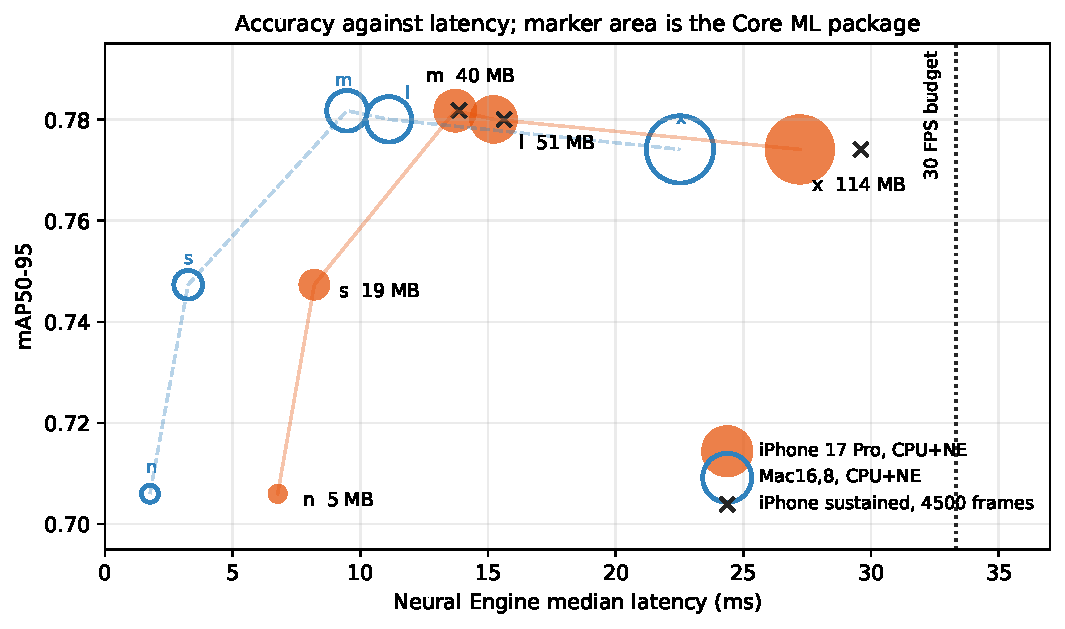
\includegraphics[width=\columnwidth]{accuracy_vs_latency.pdf}
  \caption{mAP50--95 against Neural Engine latency on both devices. Marker area
is the Core ML package size; crosses mark the sustained runs.}
  \label{fig:accuracy-latency}
\end{figure}

\subsection{Laptop and smartphone measurements are not interchangeable}

\begin{table}[t]
\caption{Median inference latency on both devices, FPS in brackets, FP16 Core
ML on identical images. The last column is the Neural Engine speed-up over the
phone's own CPU.}
\label{tab:devices}
\centering
\begin{tabular}{lrrrr}
\toprule
 & \multicolumn{2}{c}{CPU only} & \multicolumn{2}{c}{CPU + Neural Engine} \\
\cmidrule(lr){2-3}\cmidrule(lr){4-5}
Model & Mac & iPhone & Mac & iPhone \\
\midrule
YOLO11n & 9.1 (110) & 13.6 (74) & 1.76 (570) & 6.76 (148) \\
YOLO11s & 17.0 (59) & 26.1 (38) & 3.25 (307) & 8.20 (122) \\
YOLO11m & 32.4 (31) & 49.0 (20) & 9.48 (106) & 13.72 (73) \\
YOLO11l & 42.2 (24) & 59.0 (17) & 11.11 (90) & 15.22 (66) \\
YOLO11x & 69.1 (14) & 112.0 (9) & 22.51 (44) & 27.21 (37) \\
\bottomrule
\end{tabular}
\end{table}

\begin{figure*}[t]
  \centering
  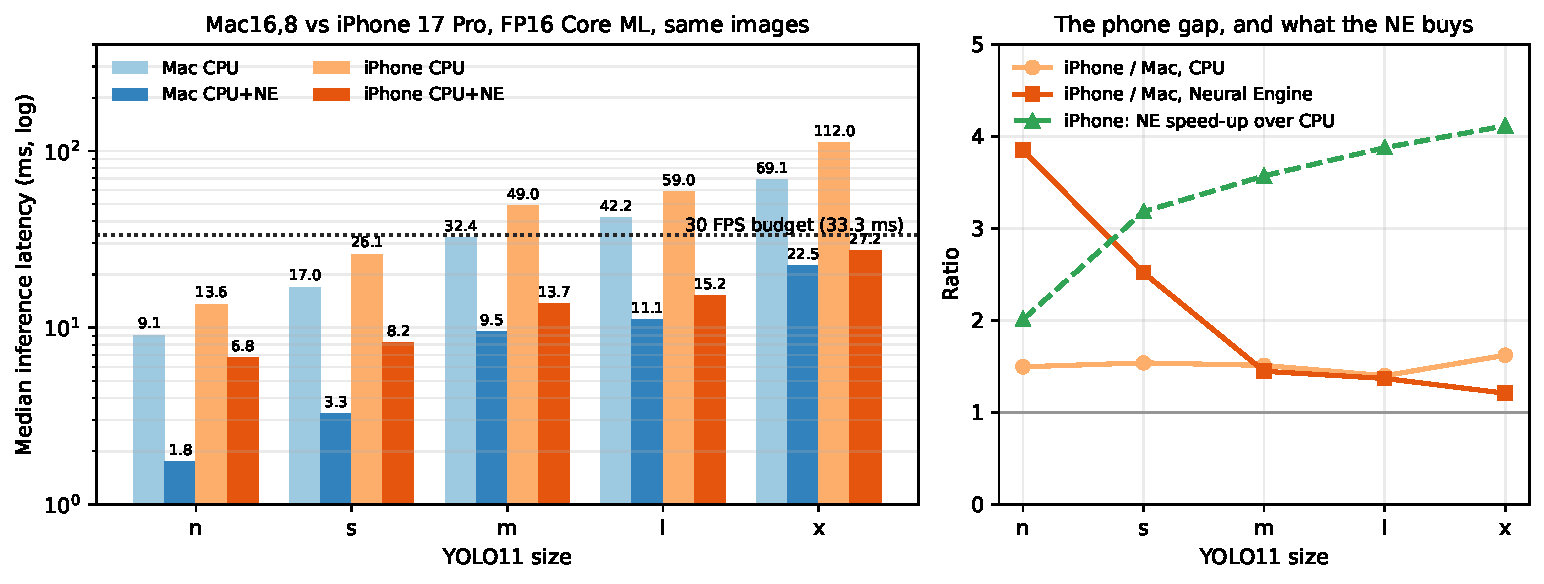
\includegraphics[width=\textwidth]{device_latency.pdf}
  \caption{Inference latency for every size on both devices and both compute
  unit settings, against a 33.3\,ms frame budget (left), and the resulting
  ratios (right). The laptop-to-phone gap is flat on the CPU and closes with
  model size on the Neural Engine.}
  \label{fig:device-latency}
\end{figure*}

The ratio between laptop and smartphone latency varies with model size
(Table~\ref{tab:devices}, Figure~\ref{fig:device-latency}). On the CPU, the
smartphone latency is 1.40 to 1.62 times the laptop latency at every size. On
the Neural Engine, the ratio is 3.85$\times$ for YOLO11n and falls monotonically
to 1.21$\times$ for YOLO11x. The Neural Engine speed-up over the smartphone's
own CPU increases with model size, from 2.0$\times$ for n to 4.1$\times$ for x.

This pattern is consistent with a fixed per-inference overhead on the
smartphone, although the benchmark does not isolate that overhead directly. A
fixed overhead would have the largest proportional effect on the smallest
model. Regardless of its cause, the measured laptop latency understates the
smartphone latency most strongly for the small models considered for mobile
deployment.

\begin{table}[t]
\caption{Each size against a 30\,FPS camera budget on the phone's Neural
Engine. The sustained column is a 4{,}500-frame run; YOLO11m's sustained figure
was collected on the earlier OS version and is not comparable with its own
short run. YOLO11n and s were not run sustained (n/r), since their short-run
p90 already leaves a margin of more than three times the budget.}
\label{tab:budget}
\centering
\begin{tabular}{lrrrl}
\toprule
Model & median & p90 & budget/p90 & sustained \\
\midrule
YOLO11n & 6.76 & 7.91 & 4.22$\times$ & n/r \\
YOLO11s & 8.20 & 10.52 & 3.17$\times$ & n/r \\
YOLO11m & 13.72 & 15.32 & 2.18$\times$ & 13.86 (72.2 FPS) \\
YOLO11l & 15.22 & 16.68 & 2.00$\times$ & 15.63 (64.0 FPS) \\
YOLO11x & 27.21 & 28.30 & 1.18$\times$ & 29.60 (33.8 FPS) \\
\bottomrule
\end{tabular}
\end{table}

Accuracy stops improving at m, while the real-time limit occurs three sizes
later. YOLO11x only narrowly meets the smartphone budget: 36.7\,FPS in a short
run, 33.8\,FPS sustained over 4{,}500 frames, and a p90 of 31.8\,ms against a
33.3\,ms budget (Table~\ref{tab:budget}). Its sustained median is 8.8\% above
its short-run median, the largest drift in the ladder. YOLO11l drifts 2.7\%,
and the reported thermal state remains \emph{fair} or better throughout. A
warmer smartphone, a larger input, or processing outside inference would cause
YOLO11x to exceed the budget.

If the Neural Engine is unavailable and the application falls back to the CPU,
as the shipped build did because of an unrelated compiler assertion on the GPU
path, the larger models fail to meet the budget three sizes earlier. YOLO11s is
the last size above 30\,FPS at 38.3; m runs at 20.4, and x runs at 8.9.

Cross-device outputs agree closely. Across all five sizes every matched box has
a mean IoU between 0.990 and 1.000 with its laptop counterpart and an identical
stage label. Two borderline boxes out of roughly thirty differ in count, which
is the same order of disagreement observed between compute units on one device.
The latency differences are therefore unlikely to result from different
detections.

Between the two measurement days the iPhone was updated from iOS~26.5.2 to
iOS~27.0. YOLO11n's Neural Engine latency changed from 4.05\,ms to
6.4--6.8\,ms across that update, repeatably, while YOLO11m was unchanged at
13.5--13.7\,ms and CPU-only latency was unchanged for both. A 67\% regression
for the smallest model, with no corresponding change for a larger model, is
further evidence of a fixed overhead instead of a change in compute throughput.
An on-device latency result therefore requires the OS version for
interpretation.
